% !TEX root = main.tex
% ================================================================

This section introduces the four methods used in our comparative study. We
first describe the two dynamic-programming baselines (DTW and Edit-distance),
then the Three-Cents recognizer, and finally the BiLSTM.
Throughout, we denote the test sequence by
$\mathcal{X} = (\mathbf{x}_1, \dots, \mathbf{x}_N)$ and a reference (template)
sequence by $\mathcal{Y} = (\mathbf{y}_1, \dots, \mathbf{y}_M)$, with
$\mathbf{x}_i, \mathbf{y}_j \in \mathbb{R}^{3}$.

% ----------------------------------------------------------------
\subsection{Dynamic Time Warping (DTW)}
% ----------------------------------------------------------------

Dynamic Time Warping is a classical technique for comparing two time-dependent
sequences that may differ in speed or duration
\cite{MyersRabiner1981}. The key idea is to find a non-linear
alignment between the two sequences that minimizes a cumulative distance,
thereby absorbing local temporal distortions.

We first define the local cost between two points $\mathbf{x}_i$ and
$\mathbf{y}_j$ via the Euclidean ($L_2$) distance:
\begin{equation}
    d(i, j) = \lVert \mathbf{x}_i - \mathbf{y}_j \rVert_2 .
\end{equation}

The accumulated distance $D(i, j)$ is then computed recursively using dynamic
programming~\cite{Rabiner1993}:
\begin{equation}
\label{eq:dtw-recurrence}
    D(i, j) = d(i, j) + \min
    \begin{cases}
        D(i-1, j-1) \\[2pt]
        D(i-1, j)   \\[2pt]
        D(i, j-1)
    \end{cases}
\end{equation}
with boundary condition $D(1, 1) = d(1, 1)$. The three candidate predecessors
correspond respectively to a diagonal step (temporal alignment), a vertical
step (the test sequence is progressing while the reference is stalling), and a
horizontal step (the reference is progressing while the test is stalling).

A warping path $W = (w_1, \dots, w_L)$, with $w_k = (i_k, j_k)$, is a sequence
of grid cells traversed from $(1,1)$ to $(N, M)$. To be physically meaningful,
$W$ must satisfy three standard constraints~\cite{Rabiner1993}:
\begin{itemize}\itemsep 0em
    \item Boundary: $w_1 = (1, 1)$ and $w_L = (N, M)$;
    \item Monotonicity: both index sequences $(i_k)$ and $(j_k)$ are
    non-decreasing (temporal order is preserved);
    \item Continuity: transitions occur only between adjacent cells, so
    that no observation is skipped.
\end{itemize}

The final similarity score $D(N, M)$ is then plugged into a $k$-nearest-neighbors classifier: the
test gesture is assigned the majority label among its $k$ closest templates.

% ----------------------------------------------------------------
\subsection{Edit-distance on quantized sequences}
% ----------------------------------------------------------------
The second baseline treats gestures as strings of discrete symbols and
classifies them using an edit-distance. The approach proceeds in two steps.
 
\paragraph{Vector quantization.} Each 3D point $\mathbf{r}(t)$ is first assigned
to one of $K$ codewords obtained by clustering the pooled training points
(via $k$-means). A gesture is thereby mapped onto a sequence of discrete
symbols $s(t) \in \{1, \dots, K\}$, turning the continuous trajectory problem
into a string-matching problem. This discretization step is necessary because
edit-distance is fundamentally a string-based metric, designed to compare
sequences of discrete elements rather than continuous coordinates.
 
\paragraph{Edit distance.} The dissimilarity between two such symbolic sequences
is measured by the Levenshtein edit distance~\cite{Levenshtein1966}, defined as
the minimum number of elementary edit operations (insertion, deletion,
substitution) required to transform one sequence into the other:
\begin{equation}
    d_{\text{ED}}(S_1, S_2) = \min \left\{ \text{cost of operations to transform } S_1 \to S_2 \right\} .
\end{equation}
 
The distance is computed using a standard dynamic-programming recursion. Let
$D(i, j)$ denote the edit distance between the first $i$ symbols of $S_1$ and
the first $j$ symbols of $S_2$. Then:
\begin{equation}
    D(i, j) = \min
    \begin{cases}
        D(i-1, j) + 1 & \text{(deletion)} \\[2pt]
        D(i, j-1) + 1 & \text{(insertion)} \\[2pt]
        D(i-1, j-1) + c(i, j) & \text{(substitution)}
    \end{cases}
\end{equation}
where $c(i, j) = 0$ if $S_1[i] = S_2[j]$, and $c(i, j) = 1$ otherwise. The
final value $D(|S_1|, |S_2|)$ gives the edit distance between the two complete
sequences. Classification is performed with a $k$-nearest-neighbors rule,
assigning each test gesture the label of its $k$ nearest templates in the
edit-distance metric.


% ----------------------------------------------------------------
\subsection{The Three-Cents recognizer}
% ----------------------------------------------------------------

The Three-Cents recognizer is a 3D specialization of the \$1 recognizer of
Wobbrock, Wilson and Li~\cite{Wobbrock2007}. The original \$1 algorithm is a
widely used gold standard for 2D gesture prototyping, relying on four steps:
\emph{resample}, \emph{rotate to a reference angle}, \emph{scale}, and
\emph{translate to the origin}, followed by template matching. While effective,
its iterative rotation search (Golden-Section Search) becomes computationally
expensive and geometrically ambiguous in 3D, where no single reference angle
exists.

Caputo et al.~\cite{Caputo2018} propose to forgo the rotation step altogether,
yielding a lightweight three-step normalization pipeline
(\emph{resample--scale--translate}) that remains robust for short mid-air
trajectories.

\subsubsection*{Three-step normalization pipeline}
 
\begin{enumerate}\itemsep 0em
    \item \textbf{Resampling.} The raw trajectory is resampled into $n$
    equidistant points along its arc length (typically $n = 64$, as in the
    original \$1 paper). This makes the representation invariant to the
    execution speed.
 
    \item \textbf{Scaling.} The resampled gesture is rescaled using a
    uniform scaling by total arc length. Let $L$ denote the total
    arc-length of the resampled trajectory:
    \begin{equation}
        L = \sum_{i=1}^{n-1} \lVert \mathbf{r}'_{i+1} - \mathbf{r}'_{i} \rVert_2 .
    \end{equation}
    Following~\cite{Caputo2018}, each point is then divided by $L$:
    \begin{equation}
        \mathbf{r}''_i = \frac{\mathbf{r}'_i}{L} .
    \end{equation}
    This choice differs from the bounding-box scaling used in the original
    \$1 algorithm, which stretches each axis independently and can distort
    the gesture shape. Uniform length-based scaling preserves the
    proportions of the trajectory, making two gestures of the same shape but
    different sizes comparable while preserving directional information
    (crucial for 3D mid-air gestures where orientation is
    discriminative)~\cite{Caputo2018}.
 
    \item \textbf{Translation.} Finally, the gesture is translated so that its
    centroid lies at the origin (0, 0, 0),
    \begin{equation}
        \mathbf{r}_{c} = \tfrac{1}{n} \sum_{i=1}^{n} \mathbf{r}'_i ,
        \qquad
        \mathbf{r}^{\text{final}}_{i} = \mathbf{r}'_i - \mathbf{r}_{c} ,
    \end{equation}
    ensuring position invariance.
\end{enumerate}

\subsubsection*{Classification}

After normalization, the candidate gesture $C = (\mathbf{c}_1, \dots,
\mathbf{c}_n)$ is compared to each template $T = (\mathbf{t}_1, \dots,
\mathbf{t}_n)$ by the average Euclidean point-to-point distance:
\begin{equation}
    D(C, T) = \frac{1}{n} \sum_{i=1}^{n}
    \lVert \mathbf{c}_i - \mathbf{t}_i \rVert_2 .
\end{equation}
A 1-Nearest-Neighbor rule is then applied: the candidate is assigned the label
of the template achieving the minimum distance. By omitting the rotation step
and relying on a fixed point-to-point correspondence, the Three-Cents
recognizer provides a ``cheap'' alternative to alignment-based methods such as
DTW, at the cost of sensitivity to global rotations.

% ----------------------------------------------------------------
\subsection{Bidirectional LSTM}
\label{sec:bilstm}
% ----------------------------------------------------------------

Unlike the previous methods, which are distance-based, the last approach
relies on a recurrent neural network that learns its representation directly
from the data. Recurrent Neural Networks (RNNs) process a sequence
$\mathcal{X} = (\mathbf{x}_1, \dots, \mathbf{x}_T)$ by maintaining a hidden
state that propagates information forward in time. Standard RNNs trained by
back-propagation through time suffer however from the
\emph{vanishing/exploding gradient problem}: the influence of an early time
step on the loss decays (or blows up) exponentially with the temporal
distance, making it practically impossible to learn long-range dependencies
\cite{Hochreiter1997, Goodfellow2016}. Since a gesture trajectory typically
spans several dozens of frames whose global shape is the primary
discriminating cue, this is a critical limitation.

\subsubsection*{LSTM cell}

The Long Short-Term Memory (LSTM) cell of Hochreiter and
Schmidhuber~\cite{Hochreiter1997} addresses this issue through an internal
\emph{cell state} $\mathbf{c}_t$, regulated by three multiplicative gates.
At each time step $t$, given the input $\mathbf{x}_t$ and the previous
hidden state $\mathbf{h}_{t-1}$:
\begin{align}
    \mathbf{f}_t &= \sigma(\mathbf{W}_f \mathbf{x}_t + \mathbf{U}_f \mathbf{h}_{t-1} + \mathbf{b}_f), \\
    \mathbf{i}_t &= \sigma(\mathbf{W}_i \mathbf{x}_t + \mathbf{U}_i \mathbf{h}_{t-1} + \mathbf{b}_i), \\
    \mathbf{o}_t &= \sigma(\mathbf{W}_o \mathbf{x}_t + \mathbf{U}_o \mathbf{h}_{t-1} + \mathbf{b}_o), \\
    \tilde{\mathbf{c}}_t &= \tanh(\mathbf{W}_c \mathbf{x}_t + \mathbf{U}_c \mathbf{h}_{t-1} + \mathbf{b}_c), \\
    \mathbf{c}_t &= \mathbf{f}_t \odot \mathbf{c}_{t-1} + \mathbf{i}_t \odot \tilde{\mathbf{c}}_t, \\
    \mathbf{h}_t &= \mathbf{o}_t \odot \tanh(\mathbf{c}_t),
\end{align}
where $\sigma$ is the logistic sigmoid, $\odot$ the element-wise product,
and $\{\mathbf{W}_\bullet, \mathbf{U}_\bullet, \mathbf{b}_\bullet\}$ are the
learned parameters. The \emph{forget gate} $\mathbf{f}_t$ controls how
much of the previous cell state is preserved, the \emph{input gate}
$\mathbf{i}_t$ how much of the candidate $\tilde{\mathbf{c}}_t$ is written
to the new state, and the \emph{output gate} $\mathbf{o}_t$ how much of the
cell state is exposed as output. The additive update of $\mathbf{c}_t$
creates a \emph{constant error carrousel} through which gradients can flow
unattenuated across many time steps, which is the key mechanism that
overcomes the vanishing gradient problem~\cite{Hochreiter1997}.
Figure~\ref{fig:lstm-cell} summarizes the cell's internal data flow.

\begin{figure}[t]
    \centering
    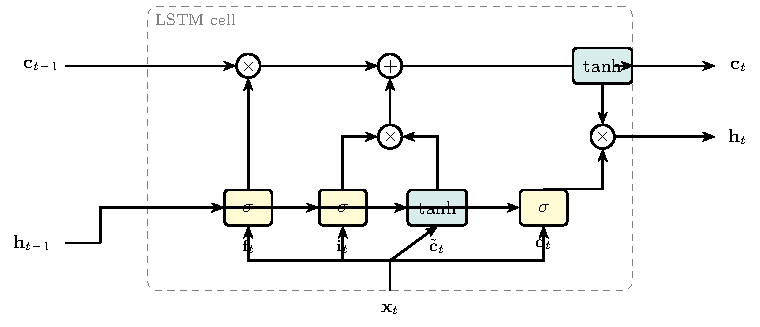
\includegraphics[width=\columnwidth]{figures/lstm_cell.pdf}
    \caption{Internal data flow of an LSTM cell. Three sigmoid gates
    ($f_t, i_t, o_t$) and one $\tanh$ candidate ($\tilde{c}_t$) jointly
    update the cell state $\mathbf{c}_t$ and produce the hidden state
    $\mathbf{h}_t$. The horizontal line carrying $\mathbf{c}_t$ acts as a
    gradient highway, enabling learning over long sequences.}
    \label{fig:lstm-cell}
\end{figure}

\subsubsection*{Bidirectional extension}

A unidirectional LSTM reads the sequence from left to right and classifies
the gesture using only the causal context up to the current frame. Since
gesture recognition is an offline task, the full trajectory is available
before any decision is made, this is unnecessarily restrictive. The
Bidirectional RNN of Schuster and Paliwal~\cite{Schuster1997} runs two
independent recurrent layers in opposite directions and concatenates their
hidden states:
\begin{equation}
    \overrightarrow{\mathbf{h}}_t = \mathrm{LSTM}_{\!\rightarrow}(\mathbf{x}_1, \dots, \mathbf{x}_t),
    \;\;
    \overleftarrow{\mathbf{h}}_t = \mathrm{LSTM}_{\!\leftarrow}(\mathbf{x}_T, \dots, \mathbf{x}_t),
\end{equation}
\begin{equation}
    \mathbf{H}_t = \left[\, \overrightarrow{\mathbf{h}}_t \,;\, \overleftarrow{\mathbf{h}}_t \,\right] \in \mathbb{R}^{2h}.
\end{equation}
Each frame is thus encoded with access to the \emph{entire} temporal
context. This is particularly useful when the beginning of a digit is
ambiguous before its closing stroke is observed (e.g., a 0 versus a 6, or
a 3 versus an 8). In our implementation each direction has $h$ hidden units
(hyperparameter \texttt{n\_units}), and only the final concatenated state
$\mathbf{H}_T$ is forwarded to the classifier head (\texttt{return\_sequences=False}).

\subsubsection*{Classifier head}

The state $\mathbf{H}_T$ is passed through a small feed-forward classifier
illustrated in Figure~\ref{fig:bilstm-arch}. Two regularization mechanisms
are applied first. \emph{Batch normalization}~\cite{Ioffe2015} rescales
each feature of $\mathbf{H}_T$ to zero mean and unit variance over the
mini-batch $\mathcal{B}$, before applying a learned affine transformation:
\begin{equation}
    \hat{y}_k = \gamma_k \,\frac{y_k - \mu_{\mathcal{B},k}}{\sqrt{\sigma^2_{\mathcal{B},k} + \varepsilon}} + \beta_k.
\end{equation}
This reduces the \emph{internal covariate shift} caused by changing
upstream weights during training, stabilizes optimization, and allows
slightly higher learning rates. \emph{Dropout}~\cite{Srivastava2014} is
then applied with rate $p = 0.30$: during training only, each activation
is independently set to zero with probability $p$, forcing the network to
learn redundant representations and acting as an implicit ensemble of
thinned sub-networks. The resulting vector is mapped through a dense layer
of $32$ ReLU units, then to a softmax over the $K = 10$ classes producing
a valid probability distribution
$p_k = e^{z_k} / \sum_{j} e^{z_j}$.

\begin{figure}[t]
    \centering
    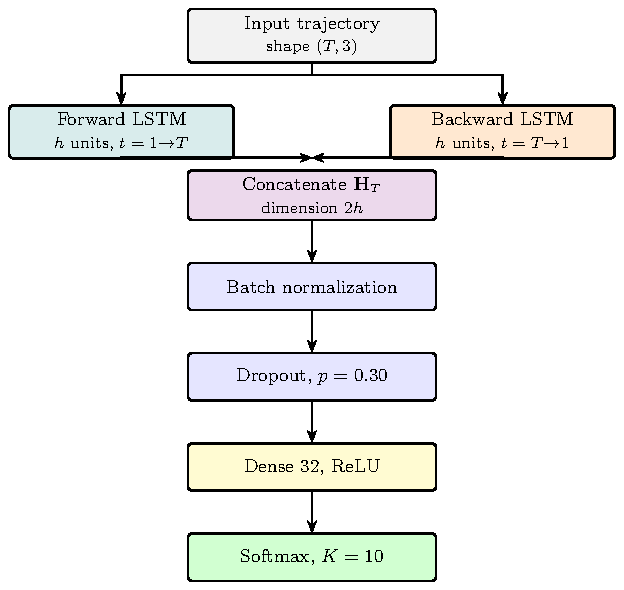
\includegraphics[width=\columnwidth]{figures/bilstm_architecture.pdf}
    \caption{Architecture of the BiLSTM classifier. The trajectory
    (resampled to $T$ points) is processed by two LSTM layers reading in
    opposite directions; their final hidden states are concatenated into
    $\mathbf{H}_T \in \mathbb{R}^{2h}$ and passed through a regularized
    classifier head producing a softmax over the $K = 10$ gesture classes.}
    \label{fig:bilstm-arch}
\end{figure}

\subsubsection*{Training}

The network is trained by minimizing the categorical cross-entropy
\begin{equation}
    \mathcal{L} = -\sum_{k=1}^{K} y_k \log p_k ,
\end{equation}
where $\mathbf{y}$ is the one-hot encoded label. Optimization uses
Adam~\cite{Kingma2015}, an adaptive first-order method that maintains
exponentially decaying estimates of the first ($\mathbf{m}_t$) and second
($\mathbf{v}_t$) moments of the gradient and adjusts the per-parameter
step size accordingly. The default hyperparameters
($\alpha = 10^{-3}$, $\beta_1 = 0.9$, $\beta_2 = 0.999$) are used. As deep
models overfit easily on the $\sim$1\,000-sample dataset, a 10\,\%
validation split is held out from each training fold to monitor validation
loss and \emph{early-stop} training when no improvement is observed for
$5$ consecutive epochs (best weights restored). Consistent with the other
methods, the model is re-initialized from scratch at every cross-validation
fold so that no information leaks between folds.